\chapter{Interval Graphs}

In this chapter an overview of the MUIG and UUIG families will be given, with their characterization.

\todo[inline]{in the case of UUIG I want to find a more exhaustive characterization using MUUIG's families to use them in TSG. In this case it will be easy to proof complexity on TSG recognition}

\section{Mixed Unit Interval Graphs}
\label{sec:muig}

\todo[inline]{Show and describe every family with demos from Joos' article}

\subsection{Families}

Here we are going to define every family of forbidden induced subgraphs for MUUIG.

\theorem\label{compaTriangular}[Gilmore, Hoffman]{A graph G is a comparability graph if and only if each odd cycle has at least one triangular chord. \cite{gilmoreCharacterizationComparabilityGraphs1964}}

An important family of forbidden induced subgraphs in paper TSG: $\mathcal{R}_k$

\begin{figure}
\begin{center}
  \begin{scaletikzpicturetowidth}{\textwidth}
  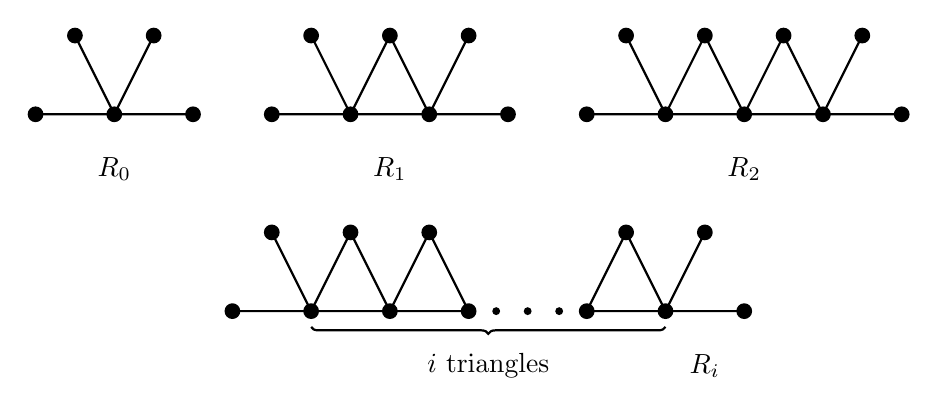
\begin{tikzpicture}[scale=1]
\def\ver{0.1} %size of a vertex
\def\x{1}

\def\xa{0.5}
\def\ya{0}

\def\xb{4}
\def\yb{0}

\def\xc{8}
\def\yc{0}

\def\xd{3.5}
\def\yd{-2.5}


%graph R_0
\path[fill] (\xa+0.5,\ya) circle (\ver);
\path[fill] (\xa+1,\ya+1) circle (\ver);
\path[fill] (\xa+2,\ya+1) circle (\ver);
\path[fill] (\xa+2.5,\ya) circle (\ver);
\path[fill] (\xa+1.5,\ya) circle (\ver);

\draw[thick] (\xa+0.5,\ya)--(\xa+1.5,\ya)--(\xa+1,\ya+1)
(\xa+2,\ya+1)--(\xa+1.5,\ya)--(\xa+2.5,\ya);

\node (1) at (\xa+1.5,\ya-0.7) {$R_0$};

%graph R_1
\path[fill] (\xb,\yb) circle (\ver);
\path[fill] (\xb+1,\yb) circle (\ver);
\path[fill] (\xb+2,\yb) circle (\ver);
\path[fill] (\xb+3,\yb) circle (\ver);
\path[fill] (\xb+0.5,\yb+1) circle (\ver);
\path[fill] (\xb+1.5,\yb+1) circle (\ver);
\path[fill] (\xb+2.5,\yb+1) circle (\ver);

\draw[thick] (\xb,\yb)--(\xb+1,\yb)--(\xb+2,\yb)--(\xb+3,\yb)
(\xb+0.5,\yb+1)--(\xb+1,\yb)--(\xb+1.5,\yb+1)--(\xb+2,\yb)--(\xb+2.5,\yb+1);

\node (1) at (\xb+1.5,\yb-0.7) {$R_1$};


%graph R_2
\path[fill] (\xc,\yc) circle (\ver);
\path[fill] (\xc+1,\yc) circle (\ver);
\path[fill] (\xc+2,\yc) circle (\ver);
\path[fill] (\xc+3,\yc) circle (\ver);
\path[fill] (\xc+4,\yc) circle (\ver);
\path[fill] (\xc+0.5,\yc+1) circle (\ver);
\path[fill] (\xc+1.5,\yc+1) circle (\ver);
\path[fill] (\xc+2.5,\yc+1) circle (\ver);
\path[fill] (\xc+3.5,\yc+1) circle (\ver);

\draw[thick] (\xc,\yc)--(\xc+1,\yc)--(\xc+2,\yc)--(\xc+3,\yc)--(\xc+4,\yc)
(\xc+0.5,\yc+1)--(\xc+1,\yc)--(\xc+1.5,\yc+1)--(\xc+2,\yc)--(\xc+2.5,\yc+1)--(\xc+3,\yc)--(\xc+3.5,\yc+1);

\node (1) at (\xc+2,\yc-0.7) {$R_2$};

%graph R_i
\path[fill] (\xd,\yd) circle (\ver);
\path[fill] (\xd+1,\yd) circle (\ver);
\path[fill] (\xd+2,\yd) circle (\ver);
\path[fill] (\xd+3,\yd) circle (\ver);
\path[fill] (\xd+4.5,\yd) circle (\ver);
\path[fill] (\xd+5.5,\yd) circle (\ver);
\path[fill] (\xd+6.5,\yd) circle (\ver);
\path[fill] (\xd+0.5,\yd+1) circle (\ver);
\path[fill] (\xd+1.5,\yd+1) circle (\ver);
\path[fill] (\xd+2.5,\yd+1) circle (\ver);
\path[fill] (\xd+5,\yd+1) circle (\ver);
\path[fill] (\xd+6,\yd+1) circle (\ver);

\fill (\xd+3.35,\yd) circle (\ver/2);
\fill (\xd+3.75,\yd) circle (\ver/2);
\fill (\xd+4.15,\yd) circle (\ver/2);

\draw[thick] (\xd,\yd)--(\xd+3,\yd)
(\xd+4.5,\yd)--(\xd+6.5,\yd)
(\xd+0.5,\yd+1)--(\xd+1,\yd)--(\xd+1.5,\yd+1)--(\xd+2,\yd)--(\xd+2.5,\yd+1)--(\xd+3,\yd)
(\xd+4.5,\yd)--(\xd+5,\yd+1)--(\xd+5.5,\yd)--(\xd+6,\yd+1);

\draw[thick,decoration={brace,mirror,raise=0.2cm},decorate] (\xd+1,\yd) -- (\xd+5.5,\yd)
node [pos=0.5,anchor=north,yshift=-0.4cm] {$i$ triangles};

\node (1) at (\xd+6,\yd-0.7) {$R_i$};

\end{tikzpicture}
\end{scaletikzpicturetowidth}
\end{center}
\caption{The class $\mathcal{R}$.}\label{graphsR}
\end{figure}

\begin{figure}
\begin{center}
  \begin{scaletikzpicturetowidth}{\textwidth}
  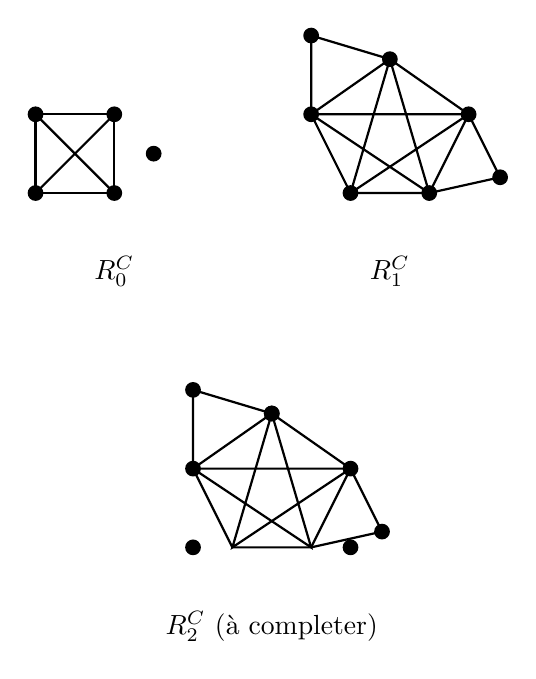
\begin{tikzpicture}[scale=1]
\def\ver{0.1} %size of a vertex
\def\x{1}

\def\xa{0.5}
\def\ya{0}

\def\xb{4}
\def\yb{0}

\def\xc{2.5}
\def\yc{-4.5}

%graph R^C_0
\path[fill] (\xa+0.5,\ya) circle (\ver);
\path[fill] (\xa+0.5,\ya+1) circle (\ver);
\path[fill] (\xa+1.5,\ya+1) circle (\ver);
\path[fill] (\xa+1.5,\ya) circle (\ver);
\path[fill] (\xa+2,\ya+0.5) circle (\ver);

\draw[thick] (\xa+0.5,\ya)--(\xa+0.5,\ya+1)--(\xa+1.5,\ya+1)
(\xa+0.5,\ya)--(\xa+1.5,\ya)--(\xa+1.5,\ya+1);
\draw[thick] (\xa+0.5,\ya)--(\xa+1.5,\ya+1);
\draw[thick] (\xa+0.5,\ya+1)--(\xa+1.5,\ya);

\node (1) at (\xa+1.5,\ya-1) {$R^C_0$};

%graph R_1
  % clique vertices
\path[fill] (\xb+1,\yb) circle (\ver);
\path[fill] (\xb+2,\yb) circle (\ver);
\path[fill] (\xb+0.5,\yb+1) circle (\ver);
\path[fill] (\xb+2.5,\yb+1) circle (\ver);
\path[fill] (\xb+1.5,\yb+1.7) circle (\ver);

  % other vertices
\path[fill] (\xb+0.5,\yb+2) circle (\ver);
\path[fill] (\xb+2.9,\yb+0.2) circle (\ver);


\draw[thick](\xb+0.5,\yb+1)--(\xb+1,\yb)--(\xb+2,\yb)--(\xb+2.5,\yb+1)--(\xb+1.5,\yb+1.7)--(\xb+0.5,\yb+1);
\draw[thick] (\xb+0.5,\yb+1)--(\xb+2,\yb)--(\xb+1.5,\yb+1.7)--(\xb+1,\yb)--(\xb+2.5,\yb+1)--(\xb+0.5,\yb+1);

\draw[thick](\xb+0.5,\yb+1)--(\xb+0.5,\yb+2)--(\xb+1.5,\yb+1.7);
\draw[thick](\xb+2.5,\yb+1)--(\xb+2.9,\yb+0.2)--(\xb+2,\yb);
\node (1) at (\xb+1.5,\yb-1) {$R^C_1$};

%graph R_2
  % clique vertices
\path[fill] (\xc+0.5,\yc) circle (\ver);
\path[fill] (\xc+2.5,\yc) circle (\ver);
\path[fill] (\xc+0.5,\yc+1) circle (\ver);
\path[fill] (\xc+2.5,\yc+1) circle (\ver);
\path[fill] (\xc+1.5,\yc+1.7) circle (\ver);
\path[fill] (\xc+1.5,\yc+1.7) circle (\ver);

  % other vertices
\path[fill] (\xc+0.5,\yc+2) circle (\ver);
\path[fill] (\xc+2.9,\yc+0.2) circle (\ver);


\draw[thick](\xc+0.5,\yc+1)--(\xc+1,\yc)--(\xc+2,\yc)--(\xc+2.5,\yc+1)--(\xc+1.5,\yc+1.7)--(\xc+0.5,\yc+1);
\draw[thick] (\xc+0.5,\yc+1)--(\xc+2,\yc)--(\xc+1.5,\yc+1.7)--(\xc+1,\yc)--(\xc+2.5,\yc+1)--(\xc+0.5,\yc+1);

\draw[thick](\xc+0.5,\yc+1)--(\xc+0.5,\yc+2)--(\xc+1.5,\yc+1.7);
\draw[thick](\xc+2.5,\yc+1)--(\xc+2.9,\yc+0.2)--(\xc+2,\yc);
\node (1) at (\xc+1.5,\yc-1) {$R^C_2$ (à completer)};


\end{tikzpicture}
\end{scaletikzpicturetowidth}
\end{center}
\caption{The class $\mathcal{R}^C$.}\label{graphsRC}
\end{figure}


\lemma{$\mathcal{R}$ is a family of co-comparability graphs.}
\proof{To prove that $\mathcal{R}$ is a family of co-comparability graphs we have to prove that its complement is a comparability graph. You can see in Figure \ref{graphsRC} the family of complements of $\mathcal{R}$ that we will call $\mathcal{R}^C$.

For this proof we will analyze the topology of $R_k^C = (V,E)$. First of all we can define two disjoint subsets $A\cup B = V$ where $\#A = k+4$ and $\#B = k+1$. $A$ is a clique and $B$ is a set of vertices such that in $R_k$ their degree is greater than 3. We can also observe that the induced subgraph $A$ is actually a tree, so there is not a cycle in $A$.

We will try to find an odd cycle $C$ such that we do not find any triangular chord in it:
\begin{itemize}
  \item $\forall_{v \in C}\ v \in A$: In this case, every cycle inside the cycle has a triangular chord.
  \item $\exists_{v \in C}\ v \in B$: In this case, we will have to find a cycle $C$ with these conditions:

  \begin{itemize}
    \item If $\#(C\cap B) \geq 3$, then a triangular chord is found.
    \item If $\#(C\cap B) = 2$, we will have to have an odd number of vertices on $A$. It can be either one (so it creates a triangulation, because both of the vertices share the same vertex in $A$) or more than 3.
    \item If $\#(C\cap B) = 1$, we will have to have an even number of vertices on $A$.
    \todo[inline]{Proof formality to be improved}
  \end{itemize}
\end{itemize}
That is, because we cannot find an odd cycle without a triangular chord, the $\mathcal{R}^C$ is a family of comparability graphs, so $\mathcal{R}$ is a family of co-comparability graphs. \qed}

\section{Unfettered Unit Interval Graphs}

\todo[inline]{Try to characterize with known forbidden families of subgraphs (from MUIG? and TSG article)}
